%%%%%%%%%%%%%%%%%%%%%%%%%%%%%%%%%%%%%%%%%%%%%%%%%%%%%%%%%%%%%%%%%%%%%%%%%%%%%%%%%%%%%%
%
% This is a pgxc_ctl tutorial.
%
% Author: Koichi Suzuki
%
% This can be disbtributed under Createve Commons Attribution-NonCommertial-SharaAlike
% 4.0 International License.
%
%%%%%%%%%%%%%%%%%%%%%%%%%%%%%%%%%%%%%%%%%%%%%%%%%%%%%%%%%%%%%%%%%%%%%%%%%%%%%%%%%%%%%%

%============= Overall Document Setting ========================================

% \documentclass{jarticle}
\documentclass[10pt,a4paper]{article}

\usepackage[dvipdfmx]{graphicx}
\usepackage{array, multirow, longtable}
\usepackage{fancyhdr}
\usepackage{fancybox}
\usepackage{booktabs}
\usepackage{url}

% Macro for long path name.
% Taken from http://www.biwako.shiga-u.ac.jp/sensei/kumazawa/tex/url.html
\newcommand{\file}{\begingroup%
	  \def\UrlBreaks{\do\\\do\/\do\_\do\-\do\+\do\=}%
		    \Url}

%=========== Additional symbols ==============================
\usepackage[T1]{fontenc}
\usepackage{textcomp}

%========== For source code listings. ========================

\usepackage{listings}
\lstset{language=c,
%  basicstyle=\ttfamily\scriptsize,
  basicstyle=\ttfamily\footnotesize,
%  commentstyle=\textit,
  commentstyle=\ttfamily,
%  classoffset=1,
  keywordstyle=\bfseries,
  frame=tRBl,
  framesep=5pt,
  showstringspaces=false,
%  numbers=left,
%  stepnumber=1,
%  numberstyle=\tiny,
  tabsize=4
}

%
% ===========================================
%    Version
%
\newcommand{\ThisVersion}{Version~1.0}
\newcommand{\ReleaseDate}{October~2$^{nd}$, 2014}

% ============================================
%    Page Format
%
\addtolength{\textwidth}{0.8in}
\addtolength{\textwidth}{1cm}
%\setlength{\topmargin}{0in}
%\addtolength{\textheight}{0.5in}
%\setlength{\oddsidemargin}{0.3in}
\setlength{\parindent}{0pt}
\setlength{\parskip}{8pt}
\setlength{\footskip}{1.2cm}
\setlength{\oddsidemargin}{1.5cm}
\setlength{\evensidemargin}{1.5cm}
\sloppy

%
% ==== Header ==================
%
\newcommand\Author[0]{Koichi Suzuki}
\newcommand\Auth[0]{K.{}Suzuki}
\pagestyle{fancy} \fancyhf{}
%\chead{\ThisVersion\quad\ReleaseDate}
% \rhead{\leftmark}
% \rhead{\ReleaseDate}
\lhead{\rightmark}
%\cfoot{Page~\thepage}
\cfoot{Page~\thepage}
\rfoot{\ThisVersion}
%\lfoot{\copyright\Author}
\lfoot{\Auth}

%
% ===========================================
%    Commonly used terms

\newcommand{\XC}{Postgres-XC}
\newcommand{\PG}{PostgreSQL}
\newcommand{\NY}{(Not implemented yet)}
\newcommand{\myjob}{Support Service of Distributed DBMS Evolvement Strategy Planning}

%
% =========================================
%	Commonly used macros
%
%\newcommand{\FUNC}[1]{\paragraph*{\file{#1}}}	% Function description
%\newcommand{\FUNC}[1]{\vspace{13pt}{\large\file{#1}}\vspace{-3pt}}	% Function description
\newcommand{\FUNC}[1]{\vspace{13pt}{\file{#1}}\vspace{-3pt}}	% Function description
%\newcommand{\Variable}[1]{\paragraph*{\file{#1} variable}} % Variable description
%\newcommand{\Variable}[1]{\vspace{13pt}{{\large\file{#1} variable:}}\vspace{-3pt} } % Variable description
\newcommand{\Variable}[1]{\vspace{13pt}{{\file{#1} variable:}}\vspace{-3pt} } % Variable description
%\newcommand{\GUC}[3]{\paragraph*{\file{#1} \quad type:\file{#2};  \quad default:\file{#3}}} % GUC
%\newcommand{\GUC}[3]{\vspace{13pt}{{\large\file{#1}} \quad type: \file{#2};  \quad default: \file{#3}}\vspace{-3pt} } % GUC
\newcommand{\GUC}[3]{\vspace{13pt}{{\file{#1}} \quad type: \file{#2};  \quad default: \file{#3}}\vspace{-3pt} } % GUC
\newcommand{\para}[1]{\par\vspace{5pt}\textbf{#1}\par}

%
% Macros for function reference table.
%
\newcommand{\FuncRefHdr}{
	\vspace{-16pt}
	\begin{center}
	\begin{tabular}[htp]{lp{0.5\hsize}} \\\hline
	Caller&File \& Description\\ \hline\vspace{3pt}
}
\newcommand{\FuncRefTrailor}{
\end{tabular}
\end{center}
}
\newcommand{\FuncRef}[3]{\file{#1}&\parbox[t]{\hsize}{\raggedright\file{#2}\\#3}}


%
% Macros to describe structure members.
%
\newcommand{\StructMemberHdr}[1]{
	\pagebreak[1]
	\begin{center}
	\file{#1} structure members\nopagebreak\\ \nopagebreak\vspace{5pt}\nopagebreak
	\begin{tabular}{lp{0.6\hsize}} \hline
	Member Name & Description\\ \hline
}
\newcommand{\AdditionalStructMemberHdr}[1]{
	\pagebreak[1]
	\begin{center}
	Additional members of \file{#1} structure\nopagebreak\\ \nopagebreak\vspace{5pt}\nopagebreak
	\begin{tabular}{lp{0.6\hsize}} \hline
	Member Name & Description\\ \hline
}
\newcommand{\StructMember}[3]{\file{#1} & \parbox[t]{\hsize}{\raggedright Type: \file{#2}; \quad #3} \\[5pt]}
\newcommand{\StructMemberTrailor}{\hline \end{tabular}\end{center}}

%
% =========================================
%	Make subsection number visible
\setcounter{secnumdepth}{3}

% ============================================
%    Title, etc.
%
\title{Pgxc\_ctl tutorial}
\date{\ReleaseDate{}}
\author{\Author}
%
% ============================================

\begin{document}

\maketitle

\newpage
\tableofcontents
\newpage

%%%%%%%%%%%%%%%%%%%%%%%%%%%%%%%%%%%%%%%%%%%%%%%%%%%%%%%%%%%%%%%%%%%%%%%%%%%%%%%%%
%
% Preface
%
%%%%%%%%%%%%%%%%%%%%%%%%%%%%%%%%%%%%%%%%%%%%%%%%%%%%%%%%%%%%%%%%%%%%%%%%%%%%%%%%%
\chapter*{Preface}

This is a tutorial document of \file{pgxc_ctl} utility.
\file{Pgxc_ctl} provides \XC cluster configuration and operation.
You can edit \file{pgxc_ctl} configuration file, initialize \XC cluster and perform
many operations such as start/stop the cluster, failover and adding/removing nodes.
Although \file{pgxc_ctl} does not provide all the potential configurations of \XC,
you can configure most of the popular configuration you may want to have.

Enjoy.

Koichi Suzuki

This article is licensed under Creative Commons
Attribution-NonCommercial-ShareAlike 4.0 International License.

\begin{flushright}
	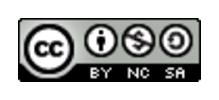
\includegraphics[width=0.15\hsize]{88x31.eps}
\end{flushright}



%%%%%%%%%%%%%%%%%%%%%%%%%%%%%%%%%%%%%%%%%%%%%%%%%%%%%%%%%%%%%%%%%%%%%%%%%%%%%%%%%
%
% PART 4: PXXC Clusaer Operations (pgxc_ctl)
%
%%%%%%%%%%%%%%%%%%%%%%%%%%%%%%%%%%%%%%%%%%%%%%%%%%%%%%%%%%%%%%%%%%%%%%%%%%%%%%%%%
\newpage

%%%%%%%%%%%%%%%%%%%%%%%%%%%%%%%%%%%%%%%%%%%%%%%%%%%%%%%%%%%%%%%%%%%%%%%%%%%%%%%%
%
% This file contains description of pgxc_ctl primer.
%
%%%%%%%%%%%%%%%%%%%%%%%%%%%%%%%%%%%%%%%%%%%%%%%%%%%%%%%%%%%%%%%%%%%%%%%%%%%%%%%%


  This section outlines how to configure and operate \XC{} database cluster through \file{pgxc_ctl}.
  \file{Pgxc_ctl} source material will be found in the \file{contrib} module of \XC{} distribution.
  Please note that \file{pgxc_ctl} does not support all the possible configurations of \XC,
  and this is mainly the reason why it is placed at \file{contrib} module, not in the main source tree.
  
  Although there are some configuration which \file{pgxc_ctl} does not support, it's a good idea
  to see what should be done in \XC{} cluster configuration and operation and what is being done in
  each operation internally.



%%%%%%%%% CHAPTER CHAPTER CHAPTER %%%%%%%%%%%%%%%%%%%%%%%%%%%%%%%%%%%%%%%%%%%%%%%%%%

\chapter{Writing configuration}


%========= SECTION SECTION ===================================================

\section{Overview of \texttt{pgxc\_ctl} configuration file and environment}

  \file{Pgxc_ctl} configuration file is in fact a \file{bash} script.
  That is, you can write any \file{bash} script which helps you to define your \XC{} configuration.
  In later sections, you will find many of such examples.
  
  Default name of the configuration file is \file{pgxc_ctl.conf}.
  You can specify other configuration file with \file{-c} option to \file{pgxc_ctl} command.
  The path is absolute or relative to \file{pgxc_ctl} directory as described in the next paragraph.
  
  \file{Pgxc_ctl} assumes dedicated directory to store its log and other materials.
  The default directory is \file{$HOME/pgxc_ctl}.
  You can change this by specifying \file{--home} option when you start \file{pgxc_ctl}.
  \file{Pgxc_ctl} has some more options to control its behavior such as log level and verbosity.
  You can specify this in ``\file{.pgxc_ctl}'' file placed in your home directory.
  Each line specifies option and its value such as:
  
  % Source Listing -------------------------------------
  \lstset{tabsize=8, xleftmargin=20pt, basicstyle=\ttfamily\scriptsize, breaklines=true}
  \begin{lstlisting}[frame=single]
[koichi@buildfarm:~]$ cat .pgxc_ctl
xc_prompt 'PGXC$ '
#verbose y
#logMessage 'DEBUG3'
#printMessage 'DEBUG1'
#printLocation y
#logLocation y
#debug y
[koichi@buildfarm:~]$
  \end{lstlisting}
  % End source Listing ---------------------------------
  
  \file{xc_prompt} is \file{pgxc_ctl} prompt in a string (it does not support serial number or other
  fancy staff as in \file{bash}l).
  Value of \file{verbose} should be \file{y} or \file{n}.
  \file{logMessage} is the level of the message goes to the log.
  You can specify \file{MANDATORY}, \file{PANIC}, \file{ERROR}, \file{WARNING}, \file{NOTICE},
  \file{NOTICE2}, \file{INFO}, \file{DEBUG1}, \file{DEBUG2} or \file{DEBUG3}.
  \file{printMessage} is the level of the message goes to the terminal you're running \file{pgxc_ctl}.
  \file{printLocation} is for debug to print location of \file{pgxc_ctl} source code with messages.
  Usually specify \texttt{n}.
  \file{Debug} also prints some more message for debugging.
  Usually, specify n.
  
  ``\file{.pgxc_ctl}'' environment file is optional.
  All the default values will be taken if no environment file is found.
  
  \file{Pgxc_ctl} log will be printed to the directory \file{pgxc_log} under \file{pgxc_ctl} directory
  unless you specify this explicitly with \file{-L} option when you start \file{pgxc_ctl}.


%========= SECTION SECTION ===================================================

\section{Get configuration file template}

  First of all, you may need configuration file template to begin with.
  You may not have \file{pgxc_ctl} directory.
  In this case, run \file{pgxc_ctl} from your home directory like this.
  
  
  % Source Listing -------------------------------------
  \begin{lstlisting}[frame=single]
[koichi@node01:~]$ pgxc_ctl prepare
Installing pgxc_ctl_bash script as /home/koichi/pgxc_ctl/pgxc_ctl_bash.
ERROR: File "/home/koichi/pgxc_ctl/pgxc_ctl.conf" not found or not a regular file. No such file or directory
Installing pgxc_ctl_bash script as /home/koichi/pgxc_ctl/pgxc_ctl_bash.
Reading configuration using /home/koichi/pgxc_ctl/pgxc_ctl_bash --home /home/koichi/pgxc_ctl --configuration /home/koichi/pgxc_ctl/pgxc_ctl.conf
Finished to read configuration.
   ******** PGXC_CTL START ***************

Current directory: /home/koichi/pgxc_ctl
[koichi@node01:~]$ ls pgxc_ctl
coordExtraConfig  pgxc_ctl.conf  pgxc_log/
[koichi@node01:~]$
  \end{lstlisting}
  % End source Listing ---------------------------------
  
  You can specify \file{pgxc_ctl} command as \file{pgxc_ctl} command line option.
  With several messages, your \file{pgxc_ctl} directory and configuration file are built.
  
  You can specify configuration file name to build as:
  
  % Source Listing -------------------------------------
  \begin{lstlisting}[frame=single]
[koichi@node01:~]$ pgxc_ctl prepare my_pgxc_ctl.conf
Installing pgxc_ctl_bash script as /home/koichi/pgxc_ctl/pgxc_ctl_bash.
ERROR: File "/home/koichi/pgxc_ctl/pgxc_ctl.conf" not found or not a regular file. No such file or directory
Installing pgxc_ctl_bash script as /home/koichi/pgxc_ctl/pgxc_ctl_bash.
Reading configuration using /home/koichi/pgxc_ctl/pgxc_ctl_bash --home /home/koichi/pgxc_ctl --configuration /home/koichi/pgxc_ctl/pgxc_ctl.conf
Finished to read configuration.
   ******** PGXC_CTL START ***************

Current directory: /home/koichi/pgxc_ctl
[koichi@node01:~]$ ls pgxc_ctl
coordExtraConfig  my_pgxc_ctl.conf  pgxc_log/
[koichi@node01:~]$ 
  \end{lstlisting}
  % End source Listing ---------------------------------
  
  Please note that you don't have to make \file{pgxc_ctl} directory.
  If not found, \file{pgxc_ctl} will make this directory when it runs.
  
  Later on, we use \file{$HOME/pgxc_ctl} as \file{pgxc_ctl} directory and \file{pgxc_ctl.conf}
  as configuration file respectively.
  Both are the default.


%========= SECTION SECTION ===================================================

\section{How configuration file looks like}

  The next figure shows the outline of \file{pgxc_ctl} configuration file.
  Details of each portion will be described later, section by section.
  Again, because the configuration file is \file{bash} script, you can use \file{bash} capability to specify specific configuration.
  You will see how template configuration uses this.
  
  % Source Listing -------------------------------------
  \begin{lstlisting}[frame=single]
#!/bin/bash
#
# Postgres-XC Configuration file for pgxc_ctl utility.
#
# Configuration file can be specified as -c option from pgxc_ctl command.   Default is
# $PGXC_CTL_HOME/pgxc_ctl.org.
#
# This is bash script so you can make any addition for your convenience to configure
# your Postgres-XC cluster.
#
# Please understand that pgxc_ctl provides only a subset of configuration which pgxc_ctl
# provide.  Here's several several assumptions/restrictions pgxc_ctl depends on.
#
...(omitted)...
# 8) Killing nodes may end up with IPC resource leak, such as semaphore and shared memory.
#    Only listening port (socket) will be cleaned with clean command.
#
# 9) Backup and restore are not supported in pgxc_ctl at present.   This is a big task and
#    may need considerable resource.
#
#========================================================================================
#
#
# pgxcInstallDir variable is needed if you invoke "deploy" command from pgxc_ctl utility.
# If don't you don't need this variable.
pgxcInstallDir=$HOME/pgxc
#---- OVERALL --------------------------------------------------------------------
#
pgxcOwner=koichi                # owner of the Postgres-XC database cluster.  Here, we use this
                                # both as lines user and database user.  This must be
                                # the super user of each coordinator and datanode.
  \end{lstlisting}
  % End source Listing ---------------------------------

  First lines are comments for the general description how the configuration file is composed.
  You may want to read this a bit carefully to avoid problems and pitfalls.

  The configuration file's goal is to specify values of pre-defined variables.


%========= SECTION SECTION ===================================================

\section{Common configuration section}

  You will see common configuration section at the top.
  In this section, you define the directory where your \XC{} binaries are installed,
  and the set of servers where you're configuring \XC{} cluster.
  
  The section looks like:
  
  % Source Listing -------------------------------------
  \begin{lstlisting}[frame=single]
# pgxcInstallDir variable is needed if you invoke "deploy" command from pgxc_ctl utility.
# If don't you don't need this variable.
pgxcInstallDir=$HOME/pgxc
#---- OVERALL ------------------------------------------------------------------
#
pgxcOwner=koichi        # owner of the Postgres-XC database cluster.  Here, we use this
                        # both as lines user and database user.  This must be
                        # the super user of each coordinator and datanode.
pgxcUser=$pgxcOwner     # OS user of Postgres-XC owner

tmpDir=/tmp                 # temporary dir used in XC servers
localTmpDir=$tmpDir         # temporary dir used here locally

configBackup=n                  # If you want config file backup, specify y to this value.
configBackupHost=pgxc-linker    # host to backup config file
configBackupDir=$HOME/pgxc      # Backup directory
configBackupFile=pgxc_ctl.bak   # Backup file name --> Need to synchronize when original changed.
  \end{lstlisting}
  % End source Listing ---------------------------------
  
  \Variable{pgxcInstallDir}
  
      First, you will find the variable \file{pgxcInstallDir|}
      This is the directory where \XC{} binaries are installed locally.
      This value is the \file{--prefix} option value of configure utility used to build
	  \XC{} binary from the source code.
      If you run make and make install, by specifying \file{--prefix} option as
	  \file{$pgxcInstallDir} value, you will have \file{$pgxcInstallDir} like this:
      
	  % Source Listing -------------------------------------
      \begin{lstlisting}[frame=single]
[koichi@buildfarm:pgxc]$ pwd
/home/koichi/pgxc
[koichi@buildfarm:pgxc]$ ls -F
bin/  include/  lib/  share/
[koichi@buildfarm:pgxc]$
      \end{lstlisting}
	  % End source Listing ---------------------------------
      
      This is used to deploy these binaries to servers with \file{deploy} command of \file{pgxc_ctl}.
      If you're installing binaries with other means, you don't have to worry about this variable.

  \Variable{pgxcOwner}
  
      Second, you will find \file{pgxcOwner} variable.
      This variable specifies owner user of \XC{} database.
  
  \Variable{pgxcUser}
  
      Next, you will find \file{pgxcUser} variable.
      This variable specifies operating system user of each server you're running \XC.
      \file{Pgxc_ctl} uses \file{ssh} for the operation of \XC{} component and assumes that
      key-based authentication is configured between the server \file{pgxc_ctl} is running
      and other servers where you run \XC{} components.
      Key-based authentication configuration is out of the scope of \file{pgxc_ctl|}
  
  \Variable{tmpDir}
  
      \file{tmpDir} variable specifies the work directory used in \file{pgxc_ctl} locally.
      Typical value can be \file{/tmp}.
      Depending upon your operating system, another value can be preferred.
      You may want to use \file{$HOME/tmp} or other user-specific directory.
  
  \Variable{localTmpDir}
  
      \file{localTmpDir} variable specifies a work directory used in the servers where you're
	  running \XC{} components.
	  \file{Pgxc_ctl} uses the same work directory among all the servers.
  
  \Variable{configBackup}
  
      \file{configBackup} variable specifies if you're backing up configuration file.
      When you change Postgres-XC cluster configuration by adding/removing nodes or promoting
	  slave to master, \file{pgxc_ctl} updates your configuration file by adding new lines to
	  specify such changes.
      If you specify the value ``\file{y}'' to this variable, \file{pgxc_ctl} will backup this
	  change to the file specified by the following variables.
      
      Although the template specifies ``\file{n},'' it specifies its backup configuration for your help.
  
  \Variable{configBackupHost}
  
      \file{configBackupHost} variable specifies what server you'd like to backup your
	  \file{pgxc_ctl} configuration file.
      It will be a good idea to backup to different server so that you can take this backup and run
	  \file{pgxc_ctl} at this server when the current \file{pgxc_ctl} server fails.
  
  \Variable{configBackupDir}
  
      \file{configBackupDir} variable specifies the directory where \file{pgxc_ctl} configuration
	  file backup is stored.
      If you don't specify ``\file{y}'' to \file{configBackup} variable, you don't have to worry
	  about this variable.
  
  \Variable{configBackupFile}
  
      \file{configBackupFile} variable specifies the file name of \file{pgxc_ctl} configuration backup.
      Unless you specify ``\file{y}'' to \file{configBackup} variable, you don't have to worry
	  about this variable.



%========= SECTION SECTION ===================================================

\section{GTM master configuration}

  Following is GTM master section of \file{pgxc_ctl} configuration template.
  It looks very simple.
  
  % Source Listing -------------------------------------
  \begin{lstlisting}[frame=single]
#---- GTM -------------------------------------------------------

# GTM is mandatory.  You must have at least (and only) one GTM master in your Postgres-XC cluster.
# If GTM crashes and you need to reconfigure it, you can do it by pgxc_update_gtm command to update
# GTM master with others.   Of course, we provide pgxc_remove_gtm command to remove it.  This command
# will not stop the current GTM.  It is up to the operator.

#---- Overall -------
gtmName=gtm

#---- GTM Master -----------------------------------------------

#---- Overall ----
gtmMasterServer=node13
gtmMasterPort=20001
gtmMasterDir=$HOME/pgxc/nodes/gtm

#---- Configuration ---
gtmExtraConfig=none         # Will be added gtm.conf for both Master and Slave (done at initialization only)
gtmMasterSpecificExtraConfig=none   # Will be added to Master's gtm.conf (done at initialization only)
  \end{lstlisting}
  % End source Listing ---------------------------------
  
  \Variable{gtmName}
  
      \file{gtmName} variable defines the node name for GTM.
      GTM master and slave shares this.
      Because we have only one GTM master in the cluster, you may not have a chance to use
	  this name in the cluster operation.
  
  \Variable{gtmMasterServer}
  
      \file{gtmMasterServer} variable is the server you are running GTM master.
  
  \Variable{gtmMasterPort}
  
      \file{gtmMasterPort} variable is TCP port number GTM uses to accept connections from
	  GTM-Proxy or coordinator/datanode backend.
      You should assign unique port number in the host \file{$gtmMasterServer}.
  
  \Variable{gtmMasterDir}
  
      \file{gtmMasterDir} variable is the work directory for GTM master.
      Similar to \PG{} server, GTM needs dedicated work directory to store its configuration file,
	  status, log and other information.
  
  %\Variable{gtmExtraConfig and gtmMasterSpecificExtraConfig}
  \vspace{13pt}{{\large\file{gtmExtraConfig} and \file{gtmMasterSpecificExtraConfig} variable:}}\vspace{-3pt}
  
      In most cases, your GTM configuration is complete with above three configuration parameters.
      \file{Pgxc_ctl} takes other configuration variables and composes GTM master configuration file.
      If you want to specify extra configuration parameter to GTM master, you can use
	  \file{gtmExtraConfig} and \file{gtmMasterSpecificExtraConfig} variable.
      
      \file{gtmExtraConfig} variable specifies the file name where additional \file{gtm.conf}
	  configuration lines are stored.
      Contents of these files will go to \file{gtm.conf} file of both GTM master and slave.
      \file{gtmMasterSpecificExtraConfig} variable specifies the file name where \file{gtm.conf}
	  configuration lines only for GTM master is stored.
      
      Details of \file{gtm.conf} file will be found at
	  \url{http://postgres-xc.sourceforge.net/docs/1_2_1/app-gtm.html}.
      Default value of these variables are set to ``\file{none},''  which means ``nothing.''
      You can specify the value ``\file{none}'' for file or server names if you don't specify any.
      
      \file{pgxc_ctl} specifies \file{listen_addresses|}, \file{port} and \file{nodename} startup
	  configuration parameters in \file{gtm.conf}.
      You should not specify these configuration values in \file{gtmExtraConfig} or
	  \file{gtmMasterSpecificExtraConfig} files.
      If you'd like to specify contents of, for example, \file{gtmExtraConfig} file, you can
	  do it by adding lines as shown below:
      
	  % Source Listing -------------------------------------
      \begin{lstlisting}[frame=single, basicstyle=\ttfamily\tiny]
#---- Configuration ---
gtmExtraConfig=gtmExtraConfig       # Will be added gtm.conf for both Master and Slave (done at initialization only)
cat > $gtmExtraConfig << EOF
log_min_messages = DEBUG1
EOF
gtmMasterSpecificExtraConfig=none   # Will be added to Master's gtm.conf (done at initialization only)
	  \end{lstlisting}
	  % End source Listing ---------------------------------

	  Because the configuration file is a \file{bash} script,  these additional lines will setup the file
	  without supplying additional files.


%========= SECTION SECTION ===================================================

\section{GTM slave configuration}

	GTM slave section of \verb|pgxc_ctl| configuration template is as follows:

	% Source Listing -------------------------------------
	\begin{lstlisting}[frame=single]
#---- GTM Slave -----------------------------------------------

# Because GTM is a key component to maintain database consistency, you may want to configure GTM slave
# for backup.

#---- Overall ------
gtmSlave=y                  # Specify y if you configure GTM Slave.   Otherwise, GTM slave will not be configured and
                            # all the following variables will be reset.
gtmSlaveServer=node12       # value none means GTM slave is not available.  Give none if you don't configure GTM Slave.
gtmSlavePort=20001          # Not used if you don't configure GTM slave.
gtmSlaveDir=$HOME/pgxc/nodes/gtm    # Not used if you don't configure GTM slave.
# Please note that when you have GTM failover, then there will be no slave available until you configure the slave
# again. (pgxc_add_gtm_slave function will handle it)

#---- Configuration ----
gtmSlaveSpecificExtraConfig=none # Will be added to Slave's gtm.conf (done at initialization only)
	\end{lstlisting}
	% End source Listing ---------------------------------

	\Variable{gtmSlave}
  
		This variable specifies if you use GTM slave.
		Specify ``\file{y}'' if you are configuring GTM slave.
		Skip this section otherwise.
  
	\Variable{gtmSlaveServer}
  
		Specify the server name you're running GTM slave.
  
	\Variable{gtmSlavePort}
  
		Specify the port number GTM slave accepts connections.
		This has to be unique in the server you specified in \file{gtmSlaveServer} variable.
  
	\Variable{ggtmSlaveDir}
  
		Specify the work directory for GTM slave.
		This has to be unique in the server you specified in \file{gtmSlaveServer} variable.
  
	\Variable{gtmSlaveSpecificExtraConfig}
  
		Specify the file name with \file{gtm.conf} configuration file entries specific to this GTM slave.
		For details of \file{gtm.conf|} please refer to
		\url{http://postgres-xc.sourceforge.net/docs/1_2_1/app-gtm.html}.
		You will find how to setup this file in the configuration file in the last section.

		\file{pgxc_ctl} specifies \file{listen_addresses}, \file{port}, and \file{nodename} startup
		configuration parameters and you should not specify these configuration values in
		\file{gtmSlaveSpecificExtraConfig} file.
 

%========= SECTION SECTION ===================================================

\section{GTM proxy configuration}
  
  GTM Proxy is not mandatory in \XC{} configuration.
  Because it provides GTM slave promotion to the master without interpreting \XC{} cluster
  operation, you may want to configure this as well unless you're configuring \XC{} locally
  for a test.
  
  It's a good idea to configure a GTM proxy, a coordinator and a datanode in a server
  balance the workloads among these components and to leverage local socket.
  
  GTM proxy configuration section looks like this:
  
  
  % Source Listing -------------------------------------
  \begin{lstlisting}[frame=single, basicstyle=\ttfamily\tiny]
#---- GTM Proxy ---------------------------------------------------------
# GTM proxy will be selected based upon which server each component runs on.
# When fails over to the slave, the slave inherits its master's gtm proxy.  It should be
# reconfigured based upon the new location.
#
# To do so, slave should be restarted.   So pg_ctl promote -> (edit postgresql.conf and recovery.conf) -> pg_ctl restart
#
# You don't have to configure GTM Proxy if you don't' configure GTM slave or you are happy if every component connects
# to GTM Master directly.  If you configure GTL slave, you must configure GTM proxy too.

#---- Shortcuts ------
gtmProxyDir=$HOME/pgxc/nodes/gtm_pxy

#---- Overall -------
gtmProxy=y      # Specify y if you configure at least one GTM proxy.   You may not configure gtm proxies
                # only when you don't' configure GTM slaves.
                # If you specify this value not to y, the following parameters will be set to default empty values.
                # If we find there're no valid Proxy server names (means, every servers are specified
                # as none), then gtmProxy value will be set to "n" and all the entries will be set to
                # empty values.
gtmProxyNames=(gtm_pxy1 gtm_pxy2 gtm_pxy3 gtm_pxy4) # No used if it is not configured
gtmProxyServers=(node06 node07 node08 node09)       # Specify none if you don't' configure it.
gtmProxyPorts=(20001 20001 20001 20001)             # Not used if it is not configured.
gtmProxyDirs=($gtmProxyDir $gtmProxyDir $gtmProxyDir $gtmProxyDir)  # Not used if it is not configured.

#---- Configuration ----
gtmPxyExtraConfig=none # Extra configuration parameter for gtm_proxy.  Coordinator section has an example.
gtmPxySpecificExtraConfig=(none none none none)
  \end{lstlisting}
  % End source Listing ---------------------------------
  
  \Variable{gtmProxyDir}
  
      This is a shortcut to specify same value for \file{gtmProxyDirs} array elements as
	  described later.
  
  \Variable{gtmProxy}
  
      \file{gtmProxy} specifies if you are configuring GTM proxy.
      Specify ``\file{y}'' if you are configuring GTM proxy.
      Specify ``\file{n}'' otherwise.
  
  \Variable{gtmProxyNames}
  
      \file{gtmProxyNames} specifies names of GTM proxies.
      Because GTM proxies are configured in more than one server, each GTM proxy need to have
	  unique name which is specified in an array.
      In this template, GTM proxy, coordinator and datanode are configured in four servers.
  
  \Variable{gtmProxyServers}
  
      \file{gtmProxyServers} specifies server for each GTM proxy.
      This is also an array.
      Specify servers for corresponding GTM proxy specified in \file{gtmProxyNames}.
  
  \Variable{gtmProxyPorts}
  
      \file{gtmProxyPorts} specifies port number of each GTM proxy.
      This is also an array like \file{gtmProxyNames}.
      Port number must be unique in each servers specified in \file{gtmProxyServers} parameter.
  
  \Variable{gtmProxyDirs}
  
      GTM proxy needs dedicated work directory.
      \file{gtmProxyDirs} parameter specifies this.
      In the template, work variable \file{gtmProxyDir} is used to assign the same value to each
	  array element.
      You can use similar way for you convenience.
  
  \Variable{gtmPxyExtraConfig}
  
      Specify the file name which contain extra \file{gtm_proxy.conf} configuration lines.
      Content of this file will go to all the \file{gtm_proxy.conf} files you are configuring.
      Specify ``\file{none}'' if you are not using this feature.
      
      Details if \file{gtm_proxy.conf} file will be found at
	  \url{http://postgres-xc.sourceforge.net/docs/1_2_1/app-gtm-proxy.html}.
      
      \file{listen_addresses},
	  \file{worker_threads} and \file{gtm_connect_retry_interval}
	  configuration options of \file{gtm_proxy.conf} 
      will be set by \file{pgxc_ctl} and you should not change them with
	  \file{gtmPxyExtraConfig} and \file{gtmPxySpecificExtraConfig}.
      
      \file{pgxc_ctl} will also setup \file{nodename|} \file{port}, \file{gtm_host}
	  and \file{gtm_port}.
      They comes at the last of \file{gtm_proxy.conf} file.
      Specifying them in \file{gtmPxyExtraConfig} or \file{gtmPxySpecificExtraConfig} will
	  not work.
  
  \Variable{gtmPxySpecificExtraConfig}
  
      You can specify extra configuration for each GTM proxy with this parameter.
      Specify file name which contains extra \file{gtm_proxy.conf} lines for each GTM proxy as
	  an element of this array.
      Specify ``\file{none}'' element value if you don't use this.


%========= SECTION SECTION ===================================================

\section{\label{pgxcCtl:coordMasterConf}Coordinator master configuration}

  If you became familiar with GTM proxy configuration, you will find coordinator and datanode
  configuration is quite similar.
  Yes, it has just a few more addition.
  
  Coordinator master configuration section looks as follows.
  Please be careful that coordinator slave configuration is at the middle of this configuration,
  which will be explained in the next section.
  
  % Source Listing -------------------------------------
  \begin{lstlisting}[frame=single, basicstyle=\ttfamily\tiny]
#---- Coordinators ----------------------------------------------------------------------------------------------------

#---- shortcuts ----------
coordMasterDir=$HOME/pgxc/nodes/coord
coordSlaveDir=$HOME/pgxc/nodes/coord_slave
coordArchLogDir=$HOME/pgxc/nodes/coord_archlog

#---- Overall ------------
coordNames=(coord1 coord2 coord3 coord4)        # Master and slave use the same name
coordPorts=(20004 20005 20004 20005)            # Master and slave use the same port
poolerPorts=(20010 20011 20010 20011)           # Master and slave use the same pooler port
coordPgHbaEntries=(192.168.1.0/24)              # Assumes that all the coordinator (master/slave) accepts
... (Omitted) ...

#---- Master -------------
coordMasterServers=(node06 node07 node08 node09)        # none means this master is not available
coordMasterDirs=($coordMasterDir $coordMasterDir $coordMasterDir $coordMasterDir)
coordMaxWALsernder=5    # max_wal_senders: needed to configure slave. If zero value is specified,
                        # it is expected to supply this parameter explicitly by external files
	                    # specified in the following.   If you don't configure slaves, leave this value to zero.
coordMaxWALSenders=($coordMaxWALsernder $coordMaxWALsernder $coordMaxWALsernder $coordMaxWALsernder)
                        # max_wal_senders configuration for each coordinator.

#---- Slave -------------
	... (omitted) ...

#---- Configuration files---
# Need these when you'd like setup specific non-default configuration 
# These files will go to corresponding files for the master.
# You may supply your bash script to setup extra config lines and extra pg_hba.conf entries 
# Or you may supply these files manually.
coordExtraConfig=coordExtraConfig   # Extra configuration file for coordinators.  
	                        # This file will be added to all the coordinators'
	                        # postgresql.conf
# Please note that the following sets up minimum parameters which you may want to change.
# You can put your postgresql.conf lines here.
cat > $coordExtraConfig <<EOF
#================================================
# Added to all the coordinator postgresql.conf
# Original: $coordExtraConfig
log_destination = 'stderr'
logging_collector = on
log_directory = 'pg_log'
listen_addresses = '*'
max_connections = 100
EOF

# Additional Configuration file for specific coordinator master.
# You can define each setting by similar means as above.
coordSpecificExtraConfig=(none none none none)
coordExtraPgHba=none    # Extra entry for pg_hba.conf.  This file will be added to all the coordinators' pg_hba.conf
coordSpecificExtraPgHba=(none none none none)
  \end{lstlisting}
  % End source Listing ---------------------------------
  
  First three variable settings for \file{coordMasterDir}, \file{coordSlaveDir} and
  \file{coordArchDir} are shortcuts to specify the same value to each array element.
  You can write any script for your convenience.
  
  \Variable{coordNames}
  
      Specify each coordinator name in this array element.
  
  \Variable{coordMasterDirs}
  
      Specify the working directory for each coordinator in this array element.
      In this template, \file{coordMasterDir} variable is used to assign the same value to
	  all the elements.
  
  \Variable{coordPorts}
  
      Specify the port number which each coordinator uses to accept connection from application or
	  other coordinators.
      This value must be unique in the server specified in \file{coordMasterServers} variable and
	  \file{coordSlaveServers} variable if you are configuring coordinator slaves.
      
      This template is based upon circular HA configuration
      where each coordinator slave runs at the next server and master and its slave uses the same port.
      Please note that each coordinator is assigned different port to meet this configuration.
  
  \Variable{poolerPorts}
  
      Coordinator implements connection pooler internally to pool connection to other coordinators and datanodes.
      This variable specifies port number which the pooler uses internally.
      The value must be unique in the server specified in \file{coordMasterServers} variable and
	  \file{coordSlaveServers} variable if you are configuring coordinator slaves,
  			
  \Variable{coordPgHbaEntries}
  			
      This is a shortcut of configuring \file{pg_hba.conf} file of each coordinator.
      Each element specified in this array will be converted into ``\texttt{host all \textit{xxx} trust}''
      format to go to \file{pg_hba.conf} where \textit{xxx} is the value of the element.
      If you don't like to have such setups, you should use \file{coordExtraPgHba} or
	  \file{coordSpecificExtraPgHba} variable.
  			
  \Variable{coordMasterServers}
  			
      This array specifies what server each coordinator runs.
  			
  \Variable{coordMasterDirs}
  			
      This array specifies work the directory of each coordinator.
      Please note that this template uses variable \file{coordMasterDir} to assign the same value to
	  each array element.
  			
  \Variable{coordMaxWalSenders}
  			
      This array specifies \file{max_wal_sender} configuration parameter value for each coordinator.
      If you are configuring coordinator slave, this value must be positive.
  			
  \paragraph*{{\tt coordExtraConfig} and {\tt coordSpecificExtraConfig}}
  			
      \file{coordextraconfig} specifies the file name which contains postgresql.conf
	  configuration entries for all the coordinators.
      The following lines are the script to set up the file.
      			
      Just like GTM proxy, you can specify \file{postgresql.conf} file entry for each coordinator
	  with \file{coordSpecificExtraConfig} array.
      Specify ``\file{none}'' for the element value if you don't use it.
      			
      \file{pgxc_ctl} will set up \file{port}, \file{pooler_port}, \file{gtm_host} and
	  \file{gtm_port} configuration at the last part of coordinator's \file{postgresql.conf} file.
      Reconfiguring these parameters using \file{coordExtraConfig} and \file{coordSpecifcExtraConig}
	  will not work.
      			
      If you are configuring coordinator slave, \file{pgxc_ctl} will configure \file{wal_level},
	  \file{archive_mode}, \file{archive_command}, and \file{max_wal_senders} as well
	  at the last part.
      Reconfiguring these parameters using \file{coordExtraConfig} and \file{coordSpecificExtraConfig}
	  will not work either in this case.
  			
  % copied and modified \Variable macro to allow two variable names
  \vspace{13pt}{{\large\file{coordExtraPgHba} and \file{coordSpecificExtraPgHba} variable:}}\vspace{-3pt} 
  			
      \file{coordExtraPgHba} specifies the file name which contains lines to go to
	  \file{pg_hba.conf} file of all the coordinators.
      			
      Each element of \file{coordSpecificExtraPgHba} array specifies the file name which contains
	  lines of \file{pg_hba.conf} file for each coordinator.


%========= SECTION SECTION ===================================================

\section{Coordinator slave configuration}

  Please note that \file{pgxc_ctl} configures coordinator slaves to use the same port as their masters.
  
  Configuration section for coordinator slave looks like this:
  
  
  % Source Listing -------------------------------------
  \begin{lstlisting}[frame=single]
#---- Slave -------------
coordSlave=y            # Specify y if you configure at least one coordinator slave.  Otherwise, the following
                        # configuration parameters will be set to empty values.
                        # If no effective server names are found (that is, every servers are specified as none),
                        # then coordSlave value will be set to n and all the following values will be set to
                        # empty values.
coordSlaveSync=y        # Specify to connect with synchronized mode.
coordSlaveServers=(node07 node08 node09 node06)         # none means this slave is not available
coordSlaveDirs=($coordSlaveDir $coordSlaveDir $coordSlaveDir $coordSlaveDir)
coordArchLogDirs=($coordArchLogDir $coordArchLogDir $coordArchLogDir $coordArchLogDir)
  \end{lstlisting}
  % End source Listing ---------------------------------
  
  \Variable{acoordSlave}
  
      Specify ``\file{y}'' if you are configuring coordinator slaves.
      Otherwise, specify ``\file{n}.''
  
  \Variable{coordSlaveSync}
  
      Specify ``\file{y}'' if you use synchronous wal shipping for the slave.
      At present, you should specify ``\file{y}'' because asynchronous wal shipping could lose some
	  transactions at promote which could make the cluster inconsistent.
  
  \Variable{coordSlaveServers}
  
      Specify which servers each coordinator slave runs.
  
  \Variable{coordSlaveDirs}
  
      Specify the work directory for each coordinator slave.
  
  \Variable{coordArchLogDirs}
  
      Specify a directory to receive WAL archive for each coordinator slave.
      

%========= SECTION SECTION ===================================================

\section{\label{pgxcCtl:datanodeMasterConf}Datanode master configuration}
      
  Datanode master and slave configuration is very similar to coordinator master and
  slave configuration.
  One major difference is that datanodes does not have the pooler.
      
  Datanode master configuration section is as follows:
    
  % Source Listing -------------------------------------
  \begin{lstlisting}[frame=single, basicstyle=\ttfamily\tiny]
#---- Datanodes -------------------------------------------------------------------------------------------------------

#---- Shortcuts --------------
datanodeMasterDir=$HOME/pgxc/nodes/dn_master
datanodeSlaveDir=$HOME/pgxc/nodes/dn_slave
datanodeArchLogDir=$HOME/pgxc/nodes/datanode_archlog

#---- Overall ---------------
#primaryDatanode=datanode1              # Primary Node.
# At present, xc has a problem to issue ALTER NODE against the primary node.  Until it is fixed, the test will be done
# without this feature.
primaryDatanode=datanode1               # Primary Node.
datanodeNames=(datanode1 datanode2 datanode3 datanode4)
datanodePorts=(20008 20009 20008 20009) # Master and slave use the same port!
datanodePgHbaEntries=(192.168.1.0/24)   # Assumes that all the coordinator (master/slave) accepts
                                        # the same connection
                                        # This list sets up pg_hba.conf for $pgxcOwner user.
                                        # If you'd like to setup other entries, supply them
                                        # through extra configuration files specified below.
# Note: The above parameter is extracted as "host all all 0.0.0.0/0 trust".   If you don't want
# such setups, specify the value () to this variable and supply what you want using datanodeExtraPgHba
# and/or datanodeSpecificExtraPgHba variables.

#---- Master ----------------
datanodeMasterServers=(node06 node07 node08 node09) # none means this master is not available.
                                                    # This means that there should be the master but is down.
                                                    # The cluster is not operational until the master is
                                                    # recovered and ready to run.   
datanodeMasterDirs=($datanodeMasterDir $datanodeMasterDir $datanodeMasterDir $datanodeMasterDir)
datanodeMaxWalSender=5                              # max_wal_senders: needed to configure slave. If zero value is 
                                                    # specified, it is expected this parameter is explicitly supplied
                                                    # by external configuration files.
                                                    # If you don't configure slaves, leave this value zero.
datanodeMaxWALSenders=($datanodeMaxWalSender $datanodeMaxWalSender $datanodeMaxWalSender $datanodeMaxWalSender)
                        # max_wal_senders configuration for each datanode

#---- Slave -----------------

	... (Omitted) ...

# ---- Configuration files ---
# You may supply your bash script to setup extra config lines and extra pg_hba.conf entries here.
# These files will go to corresponding files for the master.
# Or you may supply these files manually.
datanodeExtraConfig=none    # Extra configuration file for datanodes.  This file will be added to all the 
                            # datanodes' postgresql.conf
datanodeSpecificExtraConfig=(none none none none)
datanodeExtraPgHba=none     # Extra entry for pg_hba.conf.  This file will be added to all the datanodes' postgresql.conf
datanodeSpecificExtraPgHba=(none none none none)
  \end{lstlisting}
  % End source Listing ---------------------------------
  
  Similar to the coordinator, slave configuration is placed in the middle, which will be described in the next section.
  
  \file{datanodeMasterDir}, \file{datanodeSlaveDir} and \file{datanodeArchiLogDir} are shortcuts used
  in the following configuration.
  
  \Variable{primaryDatanode}
  
	  This configuration is unique to the datanode, specifying primary datanode name.
	  Primary datanode is the datanode where replicated table update takes place first.
	  This is how to maintain replicated table consistent.
	  In the future release of \XC, primary datanode may be determined automatically and this
	  parameter may become obsolete.
  
  \Variable{datanodeNames}
  
	  This array specifies the name of each datanode.
	  Node name of primaryDatanode has to be specified in one of the element.
  
  \Variable{datanodePorts}
  
	  Specifies the port number which datanode postmaster uses to accept connections.
	  Master and slave of each datanode uses the same port number and this number has to be
	  unique in the servers running datanode master or slave, if configured.
  
  \Variable{datanodePgHbaEntries}
  
	  Shortcut to specify \file{pg_hba.conf} file of each datanode.
	  Please see \file{CoordPgHbaEntires} description for details.
  
  \Variable{datanodeMasterServers}
  
	  This array specifies server names where each datanode master runs.
  
  \Variable{datanodeMasterDirs}
  
	  This array specifies the work directory for each datanode master.
	  This hast to be unique in the server where the coordinator master is running.
  
  \Variable{datanodeMaxWalSenders}
  
	  This array specifies \file{max_wal_senders} configuration parameter for each datanode's
	  \file{postgresql.conf}.
	  If you are configuring datanode slave, this value has to be positive.
  
  \Variable{datanodeExtraConfig}
  
	  Specify the file name which contains extra lines for postgresql.conf file of all the datanodes.
	  Specify ``\file{none}'' if you are not using this.
  
  \Variable{datanodeSpecificExtraConfig}
  
	  This array specifies the file name which contains extra lines for \file{postgresql.conf}
	  file of each corresponding datanode.
  
  \Variable{datanodeExtraPgHba}
  
	  Specify the file name which contains additional lines for \file{pg_hba.conf} file of
	  all the datanodes.
	  Specify ``\file{none}'' if you are not using this.
  
  \Variable{datanodeSpecificExtraPgHba}
  
	  This array specifies the file name which contains extra lines for \file{pg_hba.conf} of
	  each corresponding datanode.
  

%========= SECTION SECTION ===================================================

\section{Datanode slave configuration}
  
  Similar to coordinators, datanode slave uses the same port number as its master.
  
  Datanode slave configuration section looks like:
  
  
  % Source Listing -------------------------------------
  \begin{lstlisting}[frame=single, basicstyle=\ttfamily\tiny]
#---- Slave -----------------
datanodeSlave=y  # Specify y if you configure at least one coordinator slave.  Otherwise, the following
                 # configuration parameters will be set to empty values.
                 # If no effective server names are found (that is, every servers are specified as none),
                 # then datanodeSlave value will be set to n and all the following values will be set to
                 # empty values.
datanodeSlaveServers=(node07 node08 node09 node06)  # value none means this slave is not available
datanodeSlaveSync=y     # If datanode slave is connected in synchronized mode
datanodeSlaveDirs=($datanodeSlaveDir $datanodeSlaveDir $datanodeSlaveDir $datanodeSlaveDir)
datanodeArchLogDirs=( $datanodeArchLogDir $datanodeArchLogDir $datanodeArchLogDir $datanodeArchLogDir )
  \end{lstlisting}
  % End source listing -----------------------------------------
  
  \Variable{datanodeSlave}
  
	  Specify ``\file{y}'' if you are configuring datanode slaves.
	  Otherwise, specify ``\file{n}.''
  
  \Variable{datanodeSlaveServers}
  
	  This array specifies the server where each datanode slave is running.
  
  \Variable{datanodeSlaveSync}
  
	  Specify if you are using synchronous wal shipping.
	  To maintain database consistency, please specify just ``\file{y}'' here to avoid a chance to lose transactions at promotion.
  
  \Variable{datanodeSlaveDirs}
  
	  This array specifies the directory for each datanode.
  
  \Variable{datanodeArchLogDirs}
  
	  This array specifies the directory to receive each datanode's archive WAL.



%%%%%%%%% CHAPTER CHAPTER CHAPTER %%%%%%%%%%%%%%%%%%%%%%%%%%%%%%%%%%%%%%%%%%%%%%%%%%

%%%%%%%%%%%%%%%%%%%%%%%%%%%%%%%%%%%%%%%%%%%%%%%%%%%%%%%%%%%%%%%%%%%%%%%%%%%%%%%%
%
% Cluster Initialization
%
%%%%%%%%%%%%%%%%%%%%%%%%%%%%%%%%%%%%%%%%%%%%%%%%%%%%%%%%%%%%%%%%%%%%%%%%%%%%%%%%
\chapter{Initializing \XC{} cluster}

  This section describes how to initialize your \XC{} cluster.
  
  When you obtain \file{pgxc_ctl} configuration file template with \file{pgxc_ctl} prepare
  command, you have built \file{$HOME/pgxc_ctl} directory and your \file{pgxc_ctl.conf}
  file at this directory.
  
  You have designed your \XC{} configuration and edited \file{pgxc_ctl.conf} file.
  
  You have configured key-based ssh connection authentication from the computer you are running \file{pgxc_ctl}
  to each server you are running one or more \XC{} components.
  
  Now you are ready to initialize your \XC{} cluster with \file{pgxc_ctl}.


%========= SECTION SECTION ===================================================

\section{Invoke {\tt pgxc\_ctl}}

  Now invoke \file{pgxc_ctl} as your shell command.
  If \file{pgxc_ctl} does not find any error in your configuration, it will print a prompt
  asking for a command.
  
  If \file{pgxc_ctl} reports any configuration error,
  correct errors and try again.
  

%========= SECTION SECTION ===================================================

\section{\label{pgxcCtl:deploy}Deploy \XC{} binaries to servers}
  
  You should deploy all \XC{} binaries to all the servers you are running \XC{} components.
  If you have installed this by binary package or manually, you can skip this section.
  
  If you are deploying binaries with \file{pgxc_ctl}, then type \texttt{deploy all} and return.
  \file{pgxc_ctl} will visit servers where at least one \XC{} component runs
  and copy binaries to their installation directory specified in \file{pgxcInstallDir}
  configuration variable.
  
  Please note that \texttt{deploy all} does not take care of \file{PATH} environment in your shell.
  You should do this manually.


%========= SECTION SECTION ===================================================

\section{Initialize the cluster}

  Type \texttt{init all} and return.
  \file{pgxc_ctl} will do everything needed to configure and start up your \XC{}
  database cluster.
  
  Although \file{pgxc_ctl} provides more step-by-step initialization,
  this is for the test and does not provide cluster configuration using \texttt{CREAT NODE}
  statement.
  It is more convenient to use init all command.
  
  If there's something wrong, errors will be reported.
  Don't worry.
  If you need any correction to your configuration file and do it over from the scratch,
  you should do the following.
  
  \begin{enumerate}
	  \item Issue \texttt{kill all} command against \file{pgxc_ctl} command prompt to kill all the
	  		processes at servers.
		    It it doesn't work, then you should kill all the process of \file{gtm}, \file{gtm_proxy} and
			\file{postgres} manually by visiting each server.
	  \item Issue \texttt{clean all} command against \file{pgxc_ctl} prompt to clean up all the working directories.
	  \item Fix the issue in the configuration file or other settings for \file{pgxc_ctl}.
	  \item If you need to have additional servers to be involved and if you have deployed \XC{} binaries using
	  		\texttt{deploy all} command, issue \texttt{deploy \textit{newserver}} command agains \file{pgxc_ctl} prompt,
			which deploys \XC{} binaries to \textit{newserver}.
			Otherwise, install \XC{} binary in your way.
	  \item Restart this step from the beginning.
  \end{enumerate}


%========= SECTION SECTION ===================================================

\section{What {\tt init all} does}

  \texttt{Init all} command does plenty of work inside to initialize each component and configure them to work together.
  The outline is described below.
  
  \para{Initializes GTM master}

    \begin{enumerate}
		\item Kills gtm process if exists, removes the work directory if exists and then creates it.
		\item Runs initgtm utility to initialize gtm environment.
		\item Configures \file{gtm.conf} file for the master.
		\item Sets up GTM to start with appropriate GXID value.
		\item Starts GTM master
    \end{enumerate}

  \para{Initializes GTM slave if configured}

    \begin{enumerate}
		\item Kills gtm process if exists, remove work directory if exists and then create it.
		\item Runs initgtm to initialize gtm environment.
		\item Configures \verb|gtm.conf| file for the slave.
		\item Starts GTM slave.
    \end{enumerate}

  \para{Initializes GTM proxies if configured}

    The following steps are done for each gtm\_proxy in parallel.
  
    \begin{enumerate}
		\item Kills gtm\_process if exists, remove work directory if exists and them create it.
		\item Runs \file{initgtm} to initialize gtm\_proxy environment.
		\item Configures \file{gtm_proxy.conf} file.
		\item Starts GTM proxy.
    \end{enumerate}

  \para{Initializes coordinator masters}

    The following steps are done for each coordinator master in parallel.
  
    \begin{enumerate}
		\item Initializes the work directory.
		\item Runs \file{initdb} to initialize a coordinator.
		\item Configures \file{postgresql.conf} file.
		\item If coordinator slave is configured, adds wal shipping configuration to
			  \file{postgresql.conf} file.
		\item Starts coordinator master.
    \end{enumerate}

  \para{Initializes coordinator slaves if configured}

    The following steps are done for each coordinator slave in parallel.
  
    \begin{enumerate}
		\item Initializes the work directory.
		\item Runs \file{pg_basebackup} utility to build the base backup.
		\item Configures \file{recovery.conf}.
		\item Adds \file{postgresql.conf} configuration entries to run as the slave.
		\item Starts coordinator slave.
    \end{enumerate}

  \para{Initializes datanode masters}

    The following steps are done for each datanode master in parallel.
  
    \begin{enumerate}
		\item Initializes the work directory.
		\item Runs \file{initdb} to initialize a datanode.
		\item Configures \file{postgresql.conf} file.
		\item If datanode slave is configured, adds wal shipping configuration to
			  \file{postgresql.conf} file.
		\item Starts datanode master.
    \end{enumerate}

  \para{Initializes datanode slaves if configured}

    The following steps are done for each datanode slave in parallel.
  
    \begin{enumerate}
		\item Initializes the work directory
		\item Runs \file{pg_basebackup} utility to build the base backup.
		\item Configures \file{recovery.conf}.
		\item Adds \file{postgresql.conf} configuration entries to run as the slave.
		\item Starts datanode slave.
    \end{enumerate}

  \para{Configures nodes}

    \begin{enumerate}
		\item Runs \texttt{CREATE NODE} and \texttt{ALTER NODE} statement at each coordinator to
			  finalize the node configuration and make each coordinator ready to accept connections.
    \end{enumerate}



%%%%%%%%% CHAPTER CHAPTER CHAPTER %%%%%%%%%%%%%%%%%%%%%%%%%%%%%%%%%%%%%%%%%%%%%%%%%%

%%%%%%%%%%%%%%%%%%%%%%%%%%%%%%%%%%%%%%%%%%%%%%%%%%%%%%%%%%%%%%%%%%%%%%%%%%%%%%%%
%
% Building database
%
%%%%%%%%%%%%%%%%%%%%%%%%%%%%%%%%%%%%%%%%%%%%%%%%%%%%%%%%%%%%%%%%%%%%%%%%%%%%%%%%
\chapter{Build your database}

  When you are successful in init all \file{pgxc_ctl} command, you are ready to run psql or
  other utilities.
  Most of \PG{} utilities are ported to \XC.
  
  They accept \file{-h} and \file{-p} command line option to specify what coordinator to
  connect to.
  As an alternative, \file{pgxc_ctl} provides two built-in commands, \file{Createdb} and
  \file{Psql|}
  
  They choose one of the available coordinator and connect to it.
  You can specify what coordinator to connect with \file{-} followed by a coordinator name to
  connect to, not host name or port number.
  
  So you can create your own database by issuing \file{Createdb} {\it newdb} against
  \file{pgxc_ctl} prompt, or \file{pgxc_ctl} command argument.



%%%%%%%%% CHAPTER CHAPTER CHAPTER %%%%%%%%%%%%%%%%%%%%%%%%%%%%%%%%%%%%%%%%%%%%%%%%%%

%%%%%%%%%%%%%%%%%%%%%%%%%%%%%%%%%%%%%%%%%%%%%%%%%%%%%%%%%%%%%%%%%%%%%%%%%%%%%%%%
%
% Run SQL statements
%
%%%%%%%%%%%%%%%%%%%%%%%%%%%%%%%%%%%%%%%%%%%%%%%%%%%%%%%%%%%%%%%%%%%%%%%%%%%%%%%%
\chapter{Run your SQL statements}

  \file{pgxc_ctl} provides \file{Psql} built-in command which invokes psql against specified coordinator.
  You can specify the coordinator name after `\file{-}' argument like
  
  % Source listing ----------------------------------------
  \begin{lstlisting}[frame=single]
$ Psql - coord1
  \end{lstlisting}
  % End source listing ------------------------------------
  
  Where, \file{coord1} is the coordinator name.
  If you don't specify coordinator name, \file{pgxc_ctl} will choose one.
  You can specify any other psql command options too.
  
  Then you can issue any coordinator \XC{} SQL statements.

%%%%%%%%% CHAPTER CHAPTER CHAPTER %%%%%%%%%%%%%%%%%%%%%%%%%%%%%%%%%%%%%%%%%%%%%%%%%%

%%%%%%%%%%%%%%%%%%%%%%%%%%%%%%%%%%%%%%%%%%%%%%%%%%%%%%%%%%%%%%%%%%%%%%%%%%%%%%%%
%
% Writing Apps
%
%%%%%%%%%%%%%%%%%%%%%%%%%%%%%%%%%%%%%%%%%%%%%%%%%%%%%%%%%%%%%%%%%%%%%%%%%%%%%%%%
\chapter{Writing applications}

  \XC's libpq interface is binary compatible with PG~ so you can write your application with
  the same manner as \PG.
  Because of the clustering nature, there are several SQL statements which \XC{} does not support.
  Also, there are several SQL statements specific to \XC.
  For details, please refer to \XC{} document at \url{http://postgres-xc.sourceforge.net/docs/1_1/}
  or \url{http://postgres-xc.sourceforge.net/docs/1_2_1/}.

%%%%%%%%% CHAPTER CHAPTER CHAPTER %%%%%%%%%%%%%%%%%%%%%%%%%%%%%%%%%%%%%%%%%%%%%%%%%%

%%%%%%%%%%%%%%%%%%%%%%%%%%%%%%%%%%%%%%%%%%%%%%%%%%%%%%%%%%%%%%%%%%%%%%%%%%%%%%%%
%
% Backup the cluster
%
%%%%%%%%%%%%%%%%%%%%%%%%%%%%%%%%%%%%%%%%%%%%%%%%%%%%%%%%%%%%%%%%%%%%%%%%%%%%%%%%
\chapter{\label{pgxcCtl:bkup}Backing up \XC{} cluster}


%========= SECTION SECTION ===================================================

\section{\texttt{pg\_dump} and \texttt{pg\_dumpall}}

  As in the case of \PG, \file{pg_dump} and \file{pg_dumpall} are the basic backup tool of \XC.
  You can connect to one of the coordinators using \file{-h} and \file{-p} option (sorry,
  \file{pgxc_ctl} does not provide built-in command such as \file{Pg_dump} or \file{Pg_dumpall} so far).
  This is almost the same as \PG.

  Backup is consistent and can be restored using \file{psql} or \file{pg_restore}.


%========= SECTION SECTION ===================================================

\section{WAL-shipping backup}

  You can configure \XC{} coordinator and datanode to enable WAL-shipping backup manually.
  At present, \file{pgxc_ctl} does not support this feature.
  This section does not provide any further description on it so far.
  
  \file{pgxc_ctl} provides master/slave configuration and failover of each node.
  Please use this feature now.

%%%%%%%%% CHAPTER CHAPTER CHAPTER %%%%%%%%%%%%%%%%%%%%%%%%%%%%%%%%%%%%%%%%%%%%%%%%%%

%%%%%%%%%%%%%%%%%%%%%%%%%%%%%%%%%%%%%%%%%%%%%%%%%%%%%%%%%%%%%%%%%%%%%%%%%%%%%%%%
%
% Recovery from the backup
%
%%%%%%%%%%%%%%%%%%%%%%%%%%%%%%%%%%%%%%%%%%%%%%%%%%%%%%%%%%%%%%%%%%%%%%%%%%%%%%%%
\chapter{Recovery from the backup}


%========= SECTION SECTION ===================================================

\section{Recovery with \texttt{pg\_dump} and \texttt{pg\_dumpall}}

	You can restore the database using the backup made by \file{pg_dump} or
	\file{pg_dumpall|}
	First, re-initialize your cluster and then apply the dump using \file{psql}
	(when the backup was taken in text format) or \file{pg_restore}.


%========= SECTION SECTION ===================================================

\section{Recovery from WAL shipping archive}

  For the same reason as section~\ref{pgxcCtl:bkup}, this is out of the scope of
  this section. 

%%%%%%%%% CHAPTER CHAPTER CHAPTER %%%%%%%%%%%%%%%%%%%%%%%%%%%%%%%%%%%%%%%%%%%%%%%%%%

%%%%%%%%%%%%%%%%%%%%%%%%%%%%%%%%%%%%%%%%%%%%%%%%%%%%%%%%%%%%%%%%%%%%%%%%%%%%%%%%
%
% Node Failover
%
%%%%%%%%%%%%%%%%%%%%%%%%%%%%%%%%%%%%%%%%%%%%%%%%%%%%%%%%%%%%%%%%%%%%%%%%%%%%%%%%
\chapter{Node failover}

  If you configure slave of GTM, coordinator or datanode and one of hem fails, you can promote
  the slave and switch over the master.
  
  \verb|pgxc_ctl| provides only manual promotion, not automatic failover.
  The background is as follows:
  
  \begin{enumerate}
	  \item \label{pgxcCtl:failover:enum1}Automatic failover should be integrated with other
	  		resource failover, such as server hardware, network, storage and other software
			resource including web server and application server.
	  \item \ref{pgxcCtl:failover:enum1} depends upon individual system integration/configuration
	  		and it may not be acceptable in some case to provide automatic failover system just
			within database system.
  \end{enumerate}
  
  The following sections will describe \verb|pgxc_ctl| command interface to promote slaves.


%========= SECTION SECTION ===================================================

\section{GTM slave promotion}

  When GTM master fails and you are running GTM slave, you can promote GTM slave to
  the master.
  Here is how to do it with \verb|pgxc_ctl|.
  
  \para{You have configured GTM Proxy}
  
    With GTM Proxy, you can promote GTM slave without stopping \XC{} cluster.
    If  live transactions needs to communicate with GTM while GTM master is out, they
	will be aborted but you don't have to restart nodes.
    
    First, issue \texttt{failover gtm} command at \file{pgxc_ctl} command prompt like:
    
	% Source listing ----------------------------------
	\vspace{\parskip}
    \begin{lstlisting}[basicstyle=\ttfamily\normalsize,frame=single]
PGXC$ failover gtm
    \end{lstlisting}
	% End source listing ------------------------------
    
    Then, you issue reconnect \verb|gtm_proxy all| command like:
    
	% Source listing ----------------------------------
	\vspace{\parskip}
    \begin{lstlisting}[basicstyle=\ttfamily\normalsize,frame=single]
PGXC$ reconnect gtm_proxy all
    \end{lstlisting}
	% End source listing ------------------------------
    
    With this command, all gtm\_proxies will connect to the new master.
    
    Through this step, the following will be done:
    
    \begin{enumerate}
		\item Runs \verb|gtm_ctl promote| command at gtm slave.
		\item Configures \verb|gtm.conf| of the promoted gtm so that it starts as the master
			  next time.
		\item Updates your configuration file to reflect these changes.   Backup it if specified.
    \end{enumerate}
    
    Please note that these commands does not stop old GTM master.
  
  \para{You have not configured GTM Proxy}
  
    \file{pgxc_ctl} does not provide a convenient way to deal with this situation.
    You have to do the following manually.
    
    \begin{enumerate}
  		\item Runs \file{gtm_ctl} promote command at gtm slave.
  		\item Edits \file{postgresql.conf} file so that they connect to the new gtm master.
  		\item Restarts all the coordinators and datanodes.
      \end{enumerate}
  
  
%========= SECTION SECTION ===================================================
  
\section{\label{pgxcCtl:promoteCoordSlave}Coordinator slave promotion}
  
  If any coordinator fails and it has a slave running, you can promote it.
  To do this, you should invoke \texttt{failover coordinator} command like:
  
  % Source listing ----------------------------------
  \vspace{\parskip}
  \begin{lstlisting}[basicstyle=\ttfamily\normalsize,frame=single]
PGXC$ failover coordinator coordname
  \end{lstlisting}
  % End source listing ------------------------------
  
  where \textit{coordname} is the coordinator name to promote.
  
  \file{pgxc_ctl} does the following:
  
  \begin{enumerate}
	  \item Because coordinator slave is running at a different server for the master,
	  		determines which gtm\_proxy promoting coordinator should connect.
	  \item Unregisters the coordinator from GTM.
	  \item Promotes the slave using \texttt{pg\_ctl promote} command.
	  \item Edits \file{postgresql.conf} file to reflect the change in target gtm\_proxy.
	  		If gtm\_proxy is not configured in the server, gtm will be chosen.
	  \item Issues \texttt{pg\_ctl restart} to reflect these changes.
	  \item Updates \file{pgxc_ctl} configuration file and backup it if specified.
	  \item Issues \texttt{ALTER NODE} statement and \file{pgxc_pool_reload()} function
	  		at all the coordinators to reflect this change.
  \end{enumerate}
  
  Please note that all the other coordinator masters should be running to handle
  \texttt{ALTER NODE} statement.


%========= SECTION SECTION ===================================================

\section{Datanode slave promotion}

  If any datanode fails and it has a slave running, you can promote it.
  To do this, you should invoke failover datanode command like:
  
  % Source listing ----------------------------------
  \vspace{\parskip}
  \begin{lstlisting}[basicstyle=\ttfamily\normalsize,frame=single]
PGXC$ failover datanode datanodename
  \end{lstlisting}
  % End source listing ------------------------------
  
  where {\it datanodename} is the datanode name to promote.
  
  \file{pgxc_ctl} will do the following:
  
  \begin{enumerate}
	  \item Because datanode slave is running at a different server for the master,
	  		determines which gtm\_proxy promoting datanode should connect.
	  \item Unregisters the datanode from GTM.
	  \item Promotes the slave using \texttt{pg\_ctl promote} command.
	  \item Edits \file{postgresql.conf} file to reflect the change in target gtm\_proxy.
	  		If gtm\_proxy is not configured in the server, gtm will be chosen.
	  \item Issues \texttt{pg\_ctl restart} to reflect these changes.
	  \item Updates \file{pgxc_ctl} configuration file and backup it if specified.
	  \item Issues \texttt{ALTER NODE} statement and \file{pgxc_pool_reload()} function at all
	  		the coordinators to reflect this change.
  \end{enumerate}
  
  Please note that all the coordinator masters should be running to handle \verb|ALTER NODE| statement.


%%%%%%%%% CHAPTER CHAPTER CHAPTER %%%%%%%%%%%%%%%%%%%%%%%%%%%%%%%%%%%%%%%%%%%%%%%%%%

%%%%%%%%%%%%%%%%%%%%%%%%%%%%%%%%%%%%%%%%%%%%%%%%%%%%%%%%%%%%%%%%%%%%%%%%%%%%%%%%
%
% Node Addition
%
%%%%%%%%%%%%%%%%%%%%%%%%%%%%%%%%%%%%%%%%%%%%%%%%%%%%%%%%%%%%%%%%%%%%%%%%%%%%%%%%
\chapter{Adding nodes}

  \file{pgxc_ctl} provides series of command to add nodes.
  While adding a node, you don't have to stop the whole \XC{} cluster but some node may
  need restart.
  This section describes the basics of each node addition.


%========= SECTION SECTION ===================================================

\section{Adding GTM slave}

  If you did not configure GTM slave or you don't have GTM slave because original GTM slave has
  been promoted to the master, you can add GTM slave to your Postgres-XC cluster.
  
  \file{pgxc_ctl} provides \texttt{add gtm slave} command for this purpose.
  The syntax of the command is as follows:
  
  % Source listing ----------------------------------
  \vspace{\parskip}
  \begin{lstlisting}[basicstyle=\ttfamily\normalsize,frame=single]
PGXC$ add gtm slave name host port dir
  \end{lstlisting}
  % End source listing ------------------------------
  
  {\it name}, {\it host}, {\it port}, and {\it dir} are the node name, host where GTM slave
  runs, port assigned to GTM slave to accept connections and its working directory, respectively.
  
  Adding GTM slave does not affect active transactions.
  
  When adding GTM slave, \verb|pgxc_ctl| does the following:
  
  \begin{enumerate}
	  \item Updates pgxc\_ctl configuration file and backup if specified.
	  \item Initializes gtm slave and start it.
  \end{enumerate}


%========= SECTION SECTION ===================================================

\section{What about GTM master?}

  GTM master is \XC's vital component and it has to be configured and running.
  \file{pgxc_ctl} does not provide a means to ``\textbf{add}'' GTM master.
  To move GTM master to other server, run gtm slave at the target server and promote it.
  

%========= SECTION SECTION ===================================================

\section{\label{pgxcCtl:gtmProxyAddition}Adding a GTM proxy}
  
  If you are adding coordinator or datanode at a server where gtm\_proxy is not configured,
  you may want to add gtm\_proxy at this server.
  
  You can do this by issuing \texttt{add gtm\_proxy} command like:
  
  % Source listing ----------------------------------
  \vspace{\parskip}
  \begin{lstlisting}[basicstyle=\ttfamily\normalsize,frame=single]
PGXC$ add gtm_proxy name host port dir
  \end{lstlisting}
  % End source listing ------------------------------
  
  {\it name}, {\it host}, {\it port}, and {\it dir} are the node name, host where the GTM
  proxy runs, port assigned to GTM proxy to accept connections and its working directory,
  respectively.
  
  If you have not installed \XC{} binary to the server, you should do it as described in the
  Section~\ref{pgxcCtl:deploy}.
  
  When adding GTM proxy, \file{pgxc_ctl} will do the following:
  
  \begin{enumerate}
	  \item Update pgxc\_ctl configuration file and backup it if specified.
	  \item Configure GTM proxy and start it. 
  \end{enumerate}

% ---------------- WIP proofreading, Koichi, 7th Aug, 2014 -----------------------------

%========= SECTION SECTION ===================================================

\section{\label{pgxcCtl:addCoordMaster}Adding a coordinator master}

  If you have not installed \XC{} binary to the server, you should do it as described in
  the section~\ref{pgxcCtl:deploy}.
  
  If you are adding a coordinator master at a server where GTM proxy is not configured,
  you may want to configure it first, as described in the section~\ref{pgxcCtl:gtmProxyAddition}.
  
  Adding a coordinator master in \verb|pgxc_ctl| is simple.
  Just invoke \verb|add coordinator master| command like:
  
  % Source listing ----------------------------------
  \begin{lstlisting}[frame=single]
PGXC$ add coordinator master name host port pooler dir
  \end{lstlisting}
  % End source listing ------------------------------
  
  {\it name}, {\it host}, {\it port}, {\it pooler}, {\it dir} are
  the node name,
  host where the new coordinator master runs,
  port assigned to the coordinator to accept connections,
  port assigned to coordinator connection pooler,
  and its working directory, respectively.
  
  When adding a coordinator master, \verb|pgxc_ctl| will do the following:
  
  \begin{enumerate}
	  \item Update pgxc\_ctl configuration file and back up it if specified.
	  \item Initialize the working directory and run \verb|initdb| to for initial configuration of
	  		the new coordinator master.
	  \item Determine GTM proxy or GTM to use and update new coordinator master's
	  		\verb|postgresql.conf| file.
	  \item Edit \verb|pg_hba.conf| file to accept minimum connection specified in
	  		\verb|coordPgHbaEntries| variable.  See section~\ref{pgxcCtl:coordMasterConf}
			for details.
	  \item \label{addCoordMaster:5}Choose an active coordinator and issue
	  		\verb|pgxc_lock_for_backup()| to block DDL issued to all the active
			coordinators.
	  \item \label{addCoordMaster:6}Choose an active coordinator and issue \verb|pg_dumpall|
	  		to dump all the catalog information to be imported to the new coordinator master.
	  \item Start the new coordinator master with \verb|-Z restoremode| and import the catalog
	  		exported at the step \ref{addCoordMaster:6}.
	  \item Stop the new coordinator and start it with \verb|-Z coordinator| option as a coordinator.
	  \item Issue \verb|CREATE NODE| or \verb|ALTER NODE| and then \verb|pgxc_pool_reload()| at
	  		all the coordinators to reflect the change.
	  \item Close the session opened in the step \ref{addCoordMaster:5} to release DDL lock.
  \end{enumerate}


%========= SECTION SECTION ===================================================

\section{\label{pgxcCtl:addCoordSlave}Adding a coordinator slave}

  Please consider to install \XC{} binaries and configure GTM proxy as described in the
  section~\ref{pgxcCtl:addCoordMaster}.
  
  You can add a coordinator slave just as follows:
  
  % Source listing ----------------------------------
  \begin{lstlisting}[frame=single]
PGXC$ add coordinator slave name host dir archDir
  \end{lstlisting}
  % End source listing ------------------------------
  
  {\it name}, {\it host}, {\it dir} and {\it archDir} are the node name, host where the new
  coordinator slave runs, its working directory and the directory to receive WAL archive from
  its master, respectively.
  
  When adding a coordinator slave, \verb|pgxc_ctl| will do the following:
  
  \begin{enumerate}
	  \item Initialize the working directory and archive WAL directory.
	  \item \label{pgxcCtlAddCoordSlaveStep:2}Reconfigure the master's \verb|postgresql.conf|
	  		file to begin WAL shipping.
	  \item \label{pgxcCtlAddCoordSlaveStep:3}Reconfigure the master's \verb|pg_hba.conf|
	  		file to accept WAL shipping connection from the new slave.
	  \item Update pgxc\_ctl configuration file and backup it if specified.
	  \item Restart the master to reflect changes done in \ref{pgxcCtlAddCoordSlaveStep:2} and
	  		\ref{pgxcCtlAddCoordSlaveStep:3}.
	  \item Run \verb|pg_basebackup| to build the master's base backup at the slave's work
	  		directory to start with.
	  \item Update the slave's \verb|postgresql.conf| to run as a slave.
	  \item Configure the slave's \verb|recovery.conf| file to connect to the master for log shipping.
	  \item Start the slave.
  \end{enumerate}



%========= SECTION SECTION ===================================================

\section{Adding a datanode master}

  Adding a datanode master is similar to adding a coordinator master as described in the
  section~\ref{pgxcCtl:addCoordMaster}.
  Please consider to install Postgres-XC binaries and GTM proxy if needed, as described in
  the section~\ref{pgxcCtl:deploy}.
  
  To add a datanode master, you can issue add datanode master command as follows:
  
  % Source listing ----------------------------------
  \begin{lstlisting}[frame=single]
PGXC$ add datanode master name host port dir
  \end{lstlisting}
  % End source listing ------------------------------
  
  {\it name}, {\it host}, {\it port}, and {\it dir} are the node name, host where the new
  datanode master runs, port number used to accept connections, and the working directory,
  respectively.
  
  Please note that adding a datanode master does not redistribute the table data automatically
  because you can specify a set of nodes to distribute or replicate each table.
  To redistribute tables, use \verb|ALTER TABLE| statement
  as described in \url{http://postgres-xc.sourceforge.net/docs/1\_2\_1/sql-altertable.html}
  and \url{http://postgres-xc.sourceforge.net/docs/1\_1/sql-altertable.html}.
  
  When adding a datanode master, \verb|pgxc_ctl| will do the following:
  
  \begin{enumerate}
	  \item Update pgxc\_ctl configuration file and back up it if specified.
	  \item Initialize the working directory and run \verb|initdb| to for initial configuration
	  		of the new datanode master.
	  \item Determine GTM proxy or GTM to use and update new datanode master's
	  		\verb|postgresql.conf| file.
	  \item Edit \verb|pg_hba.conf| file to accept minimum connection specified in
	  		\verb|datanodePgHbaEntries| variable.
			See section~\ref{pgxcCtl:datanodeMasterConf} for details.
	  \item \label{AddDatanodeMaster:step5}Choose an active coordinator and issue
	  		\verb|pgxc_lock_for_backup()| to block DDL issued to all the active coordinators
			\footnote{
				In the current release, {\tt pgxc\_lock\_for\_backup()} is targeted to a datanode
				master and does not propagate to other nodes.
				It should have targeted to a coordinator.
				Fix will be committed and available at the next minor release.
			}.
	  \item \label{AddDatanodeMaster:step6}Choose an active datanode and issue \verb|pg_dumpall|
	  		to dump all the catalog information to be imported to the new coordinator master.
	  \item Start the new datanode master with \verb|-Z restoremode| and import the catalog
	  		exported at the step \ref{AddDatanodeMaster:step6}.
	  \item Stop the new datanode and start it with \verb|-Z datanode| option as a datanode.
	  \item Issue \verb|CREATE NODE| and \verb|pgxc_pool_reload()| at all the coordinators to
	  		reflect the change.
	  \item Close the session opened in the step \ref{AddDatanodeMaster:step5} to release DDL lock.
  \end{enumerate}



%========= SECTION SECTION ===================================================

\section{Adding a datanode slave}

  Please note that the master datanode must be configured and running to add a datanode slave.
  Please also consider to install Postgres-XC binaries and configure GTM proxy if needed,
  as described in the section~\ref{pgxcCtl:deploy}.
  
  Adding datanode slave is quite similar to adding coordinator slave.
  You can do this as follows:
  
  % Source listing ----------------------------------
  \begin{lstlisting}[frame=single]
PGXC$ add datanode slave name host dir archDir
  \end{lstlisting}
  % End source listing ------------------------------
  
  {\it name}, {\it host}, {\it dir} and {\it archDir} are the node name, host where the new
  datanode slave runs, its working directory and the directory to receive WAL archive from
  its master, respectively.
  
  When adding a datanode slave, \verb|pgxc_ctl| will do the following:
  
  \begin{enumerate}
	  \item Initialize the working directory and archive WAL directory.
	  \item \label{AddDatanodeSlave:step2}Reconfigure the master's \verb|postgresql.conf|
	  		file to begin WAL shipping.
	  \item \label{AddDatanodeSlave:step3}Reconfigure the master's \verb|pg_hba.conf| file
	  		to accept WAL shipping connection from the new slave.
	  \item Update pgxc\_ctl configuration file and backup it if specified.
	  \item Restart the master to reflect changes done in \ref{AddDatanodeSlave:step2} and
	  		\ref{AddDatanodeSlave:step3}.
	  \item Run \verb|pg_basebackup| to build the master's base backup at the slave's work
	  		directory to start with.
	  \item Update the slave's \verb|postgresql.conf| to run as a slave.
	  \item Configure the slave's \verb|recovery.conf| file to connect to the master for
	  		log shipping.
	  \item Start the slave.
  \end{enumerate}



%%%%%%%%% CHAPTER CHAPTER CHAPTER %%%%%%%%%%%%%%%%%%%%%%%%%%%%%%%%%%%%%%%%%%%%%%%%%%

%%%%%%%%%%%%%%%%%%%%%%%%%%%%%%%%%%%%%%%%%%%%%%%%%%%%%%%%%%%%%%%%%%%%%%%%%%%%%%%%
%
% Node Removal
%
%%%%%%%%%%%%%%%%%%%%%%%%%%%%%%%%%%%%%%%%%%%%%%%%%%%%%%%%%%%%%%%%%%%%%%%%%%%%%%%%
\chapter{Removing nodes}

  As mentioned, GTM master is a vital \XC{} component and it is not allowed to remove it.
  GTM master has to be running when \XC{} cluster is running.


%========= SECTION SECTION ===================================================

\section{Removing GTM slave}

  You should stop GTM slave before removing.
  \verb|pgxc_ctl| provides command to do this:
  
  % Source listing ----------------------------------
  \begin{lstlisting}[frame=single]
PGXC$ stop gtm slave
  \end{lstlisting}
  % End source listing ------------------------------
  
  Then, you can remove GTM slave by:
  
  % Source listing ----------------------------------
  \begin{lstlisting}[frame=single]
PGXC$ remove gtm slave
  \end{lstlisting}
  % End source listing ------------------------------
  
  To remove gtm slave, \verb|pgxc_ctl| does the following:
  
  \begin{enumerate}
	  \item Update pgxc\_ctl configuration file and back up it if specified.
  \end{enumerate}


%========= SECTION SECTION ===================================================

\section{Removing GTM proxy}

  Before you remove a gtm proxy, you should stop it.
  \verb|pgxc_ctl| provides a command to do as follows:
  
  % Source listing ----------------------------------
  \begin{lstlisting}[frame=single]
PGXC$ stop gtm_proxy name
  \end{lstlisting}
  % End source listing ------------------------------
  
  where {\it name} is gtm\_proxy name to stop.
  
  Then, you can remove the gtm\_proxy as follows:
  
  % Source listing ----------------------------------
  \begin{lstlisting}[frame=single]
PGXC$ remove gtm_proxy name
  \end{lstlisting}
  % End source listing ------------------------------
  
  Please note that you should configure coordinators and datanodes connecting to this gtm
  proxy and restart them.
  It is advised that you can remove a gtm proxy if no coordinators or datanodes are connected
  to it any longer.


%========= SECTION SECTION ===================================================

  \section{\label{pgxcCtl:removeCoordMaster}Removing coordinator master}
  
  Because a coordinator does not store user data, it is not harmful to remove a coordinator master.
  Please do not issue DDL while you are removing coordinator master, or such DDL could be
  propagated to the removing coordinator.
  
  \verb|pgxc_ctl| does not care if the removing coordinator master is running.
  If it is running, \verb|pgxc_ctl| will stop it.
  
  The command to remove a coordinator master is as follows:
  
  % Source listing ----------------------------------
  \begin{lstlisting}[frame=single]
PGXC$ remove coordinator master name
  \end{lstlisting}
  % End source listing ------------------------------
  
  where {\it name} is the coordinator node name to remove.
  
  \verb|pgxc_ctl| will do the following to remove a coordinator master.
  
  \begin{enumerate}
	  \item Remove the slave of the removing coordinator master if configured.
	  		See the next section for details.
	  \item Issue \verb|DROP NODE| statement at all the other coordinator to remove
	  		the coordinator from all the other coordinators.
	  \item Stop the coordinator master if running.
	  \item Update pgxc\_ctl configuration file and back up it if specified.
  \end{enumerate}


%========= SECTION SECTION ===================================================

\section{\label{pgxcCtl:removeCoordSlave}Removing a coordinator slave}

  You can remove a coordinator slave by following \verb|pgxc_ctl| command.
  
  % Source listing ----------------------------------
  \begin{lstlisting}[frame=single]
PGXC$ remove coordinator slave name
  \end{lstlisting}
  % End source listing ------------------------------
  
  where {\it name} is the coordinator name to remove.
  
  \verb|pgxc_ctl| will do the following to remove a coordinator slave.
  
  \begin{enumerate}
	  \item If the coordinator slave is running, stop it.
	  \item Update the master's configuration to disable log shipping.
	  \item Restart the master.
	  \item Update pgxc\_ctl configuration file and back up it if specified.
  \end{enumerate}


%========= SECTION SECTION ===================================================

\section{Removing a datanode master}

  Before you remove a datanode master, please be sure that the removing datanode does not
  contain any user data.
  You can check this by using \verb|\d+| {\it pattern} command to \verb|psql|.
  Issue \verb|ALTER TABLE| statement to each table to remove the datanode from its
  replication or distribution nodes.
  
  You can remove a datanode master with the command:
  
  % Source listing ----------------------------------
  \begin{lstlisting}[frame=single]
PGXC$ remove datanode master name
  \end{lstlisting}
  % End source listing ------------------------------
  
  where {\it name} is the datanode node name to remove.
  
  \verb|pgxc_ctl| will do the following to remove a datanode master.
  
  \begin{enumerate}
	  \item If slave is configured for this mater, remove it.
	  		See the next section for details.
	  \item Issue \verb|DROP NODE| statement in all the coordinators to remove this datanode.
	  \item Update pgxc\_ctl configuration file and back up it if specified.
  \end{enumerate}


%========= SECTION SECTION ===================================================

\section{Removing a datanode slave}

  Removing a datanode slave is quite similar to removing a coordinator slave.
  You can do this by the following \verb|pgxc_ctl| command:
  
  % Source listing ----------------------------------
  \begin{lstlisting}[frame=single]
PGXC$ remove datanode slave name
  \end{lstlisting}
  % End source listing ------------------------------
  
  where {\it name} is the datanode name to remove.
  
  \verb|pgxc_ctl| will do the following to remove a datanode slave.
  
  \begin{enumerate}
	  \item If the coordinator slave is running, stop it.
	  \item Update the master's configuration to disable log shipping.
	  \item Restart the master.
	  \item Update pgxc\_ctl configuration file and back up it if specified.
  \end{enumerate}



\end{document}
